Classic routing protocols are categorised in two dimensions:
centralised/distributable and proactive/reactive.
The unique challenges inherent in wireless ad-hoc networks led to a larger
amount of categories, which are not always necessarily disjoint, meaning
that an algorithm may belong to one or more categories.

\subsection{Basics: Proactive and reactive routing}
Proactive and reactive routing algorithms are the basic dimensions of routing
categories.

\subsubsection*{Proactive routing}
In proactive routing algorithms, each router builds its routing table by
(regularly) exchanging messages with other routers in the network.

This has the advantage that routing information is already available when a
package is to be routed.
A huge disadvantage of proactive routing protocols is the overhead imposed
by the exchange of the update messages.

\subsubsection*{Reactive routing}
In a reactive routing algorithm, routes are discovered when a packet arrives
from a source and needs to be delivered to some destination.
While the routes need to be discovered more often than in proactive algorithms,
there is no traffic overhead due to the lack of special control messages, and
as such, the reactive approach is considered to scale better.

Two examples of reactive routing protocols are dynamic source routing (DSR)
and ad-hoc on-demand distance vector routing (AODV). The difference between
the two is that DSR, as a source routing protocol, records the entire route
in the package during the route discovery phase; and does not store routing
tables in the intermediate nodes, thus simplifying their design.

\subsection{Other categories}
Distinguishing between proactive and reactive routing algorithms gives a very
coarse categorisation. As such, several other categories have been identified
over the years.

\subsubsection*{Geographical routing}
The basic idea behind geographical routing is that nodes are addressed by
their geographic location instead of an IP address. This has the advantage
that each node does not need to know the full network topology, but each
node needs to know its location and each source needs to know the location
of the receiver.

In section~\ref{gaf} we will take a look at the Geographic adaptive fidelity (GAF)
protocol, which utilises geographical features for routing, although with an
interesting twist.

\subsubsection*{Geo-cast}
Geo-cast routing merges multi-cast routing with geographical routing, to
deliver messages to a group of nodes identified by their locations.

\subsubsection*{Hierarchical}
A hierarchical routing algorithm defines multiple zones or clusters with
gateways that connect them with each other. Inside a cluster, there often
are one or more cluster heads, that are responsible for maintaining the
connectivity within the cluster. Non-head nodes can only communicate with
their cluster heads, whereas gateway nodes can exchange information with
other clusters.


\subsubsection*{Multi-path}
In a multi-path routing algorithms, multiple paths exists from one source
to a destination. The obvious advantages of a multi-path routing
algorithm include fault tolerance (if one path fails, another is still in
use), load distribution (congested routes can be avoided by chosing alternative
routes), peak performance (multiple routes may be used in parallel for different
parts of data).

Energy-efficiency is not a paramount concern of most multi-path routing, the
load balancing idea can however not only be applied to performance, but also
to power levels, to distribute the power used within the network, as we will
see later on. Such an algorithm would of course also be power-aware.

\subsubsection*{Power-aware}
A power-aware routing algorithm tries to find a good trade off between
power consumption of nodes and mobility. Yu, Lee, Youn~\cite{main1} describe two categories
of power-aware protocols:

First, there are those algorims that try to minimise the \textit{active communication energy}. Two
subcategories can be identified:
\begin{itemize}
    \item Transmission power control -- controlling the power that is used for transmitting a packet
    \item Load control/balancing -- algorithms that distribute the load over available nodes
\end{itemize}
There also exist hybrids of the two, for example, DSRPA (section~\ref{dsrpa})
selects nodes with the freshest batteries and also controls the transmission
power.

Other algorithms do not try to minimise the active communication energy, but
instead focus on minimising the  \textit{inactivity (idle) power consumption}. For example, unused
nodes can be put to sleep or into lower power states. This subcategory often
distinguishes between master and slave nodes -- for example, SPAN (section~\ref{span}), but there are also protocols
where no such distinction is made -- for example, PEN (section~\ref{pen}).

\subsubsection*{Hybrid}
A hybrid protocol starts off as a proactive routing protocol but switches
to reactive routing for newly added nodes in order to reduce the control
overhead of proactive routing. In ad-hoc networks, it is implemented in
hierarchical network architectures.

\subsubsection*{Flow-oriented}
Alotaibi and Mukherjee~\cite{alotaibi2012survey} list flow-oriented or flow-aware
routing as another category.
Examples they list include
IERP, which most likely refers to the The Interzone Routing Protocol for Ad Hoc Networks, an Internet Draft\cite{manet-zone-ierp-02};
and SrcRR\cite{aguayo2005srcrr}, a wireless mesh network routing protocol. It is unclear what exactly
makes these routing protocols flow-aware, and in absence of any definition of
that term, it does not warrant any further discussion. 

\subsubsection*{WMN}
WMN routing algorithms are routing algorithms for wireless mesh networks.
A wireless mesh network is a special type of (ad-hoc) networks in which all
nodes participate in the distribution of data.

Over the years, multiple routing algorithms for wireless mesh networks have
been designed, examples include B.A.T.M.A.N. and the newer B.A.T.M.A.N. advanced
which is used in the Freifunk community, for example\cite{batman-adv}.
% OUT OF PLACE
\begin{figure*}
\centering
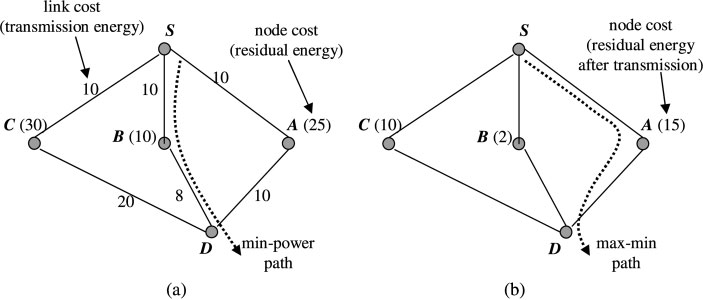
\includegraphics[width=0.7\textwidth]{images/omm}
\caption{Paths in OMM\cite{alotaibi2012survey}}
\label{ommex}
\end{figure*}
\subsubsection*{Multicast}
Multicast routing algorithms are simply routing algorithms for multicast
groups.
One example for a multicast routing algorithm is multicast ad-hoc on-demand
distance vector (MAODV)\cite{manet-maodv-00}, which is currently a work
in progress internet-draft.
